\documentclass[class=article, crop=false]{standalone}
\usepackage{my_preamble}
\begin{document}
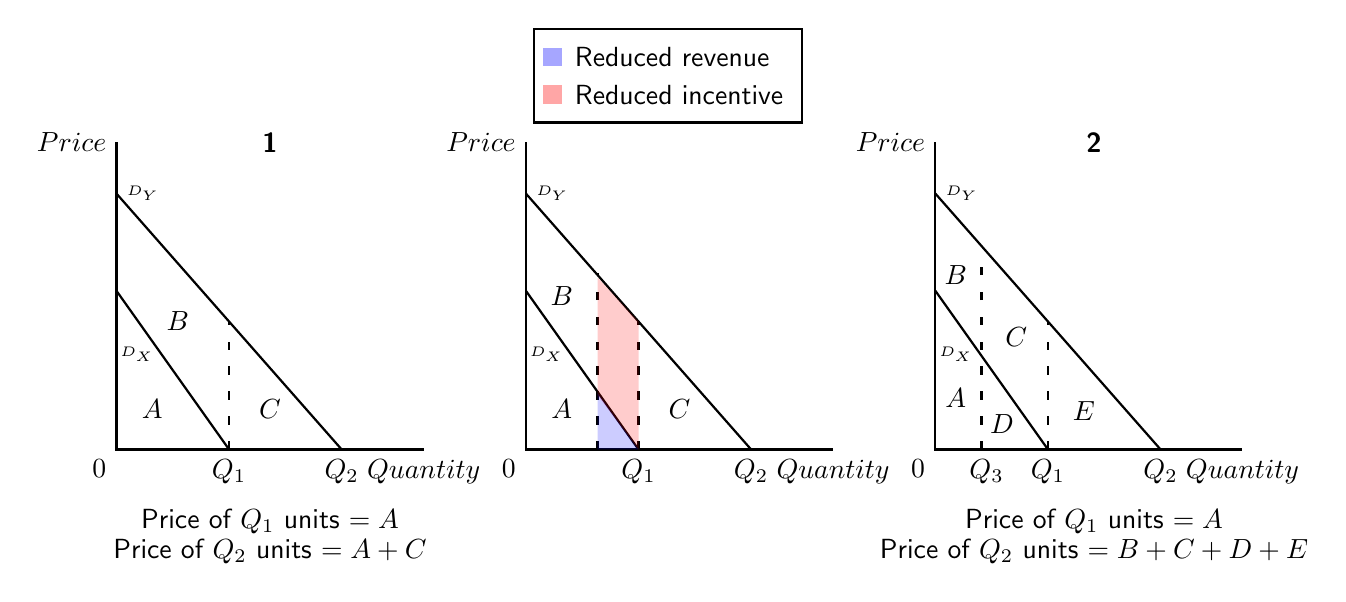
\begin{tikzpicture}[thick,font=\sffamily,scale=1.3,
  					bluenode/.style={shape=rectangle, fill=blue!35, line width=2},
  					rednode/.style={shape=rectangle, fill=red!35, line width=2}
					]
	%axies
	\draw (-6,3) node[left]{$Price$} -- (-6,0) node[below left] {$0$} -- (-3,0) node[below]{$Quantity$}; %market
	\draw (-2,3) node[left]{$Price$} -- (-2,0) node[below left] {$0$} -- (1,0) node[below]{$Quantity$}; %type 1
	\draw (2,3) node[left]{$Price$} -- (2,0) node[below left] {$0$} -- (5,0) node[below]{$Quantity$}; %type 2
	
	%titles
	%\node[] at (-4.5,2.8) {Market}; %Market title
	%\node[] at (-0.5,2.8) {Type 1}; %Type 1 title
	%\node[] at (3.5,2.8) {Type 2}; %Market title
	  
	 %market-----------------------------------------------
	\draw[] (-6,2.5) -- (-3.8,0); %demand y
	\node[right] at (-6,2.5) {\tiny{$D_{Y}$}}; %Y's Demand label
	\draw[] (-6,1.55) -- (-4.9,0); %demand x
	\node[below] at (-5.8,1.1) {\tiny{$D_{X}$}}; %X's Demand label
	\draw[loosely dashed] (-4.9,0) -- (-4.9,1.25); %separator
	\node[] at (-5.65,0.4) {$A$}; %A label
	\node[] at (-5.4,1.25) {$B$}; %B label
	\node[] at (-4.5,0.4) {$C$}; %C label
	\node[below] at (-4.9,0) {$Q_{1}$}; %Q1 label
	\node[below] at (-3.8,0) {$Q_{2}$}; %Q2 label
		
	 %Type 1 - elastic-------------------------------------
	\draw[] (-2,2.5) -- (0.2,0); %demand y
	\node[right] at (-2,2.5) {\tiny{$D_{Y}$}}; %Y's Demand label
	\draw[] (-2,1.55) -- (-0.9,0); %demand x
	\node[below] at (-1.8,1.1) {\tiny{$D_{X}$}}; %X's Demand label
	\draw[loosely dashed] (-0.9,0) -- (-0.9,1.25); %separator 1
	\draw[loosely dashed] (-1.3,0) -- (-1.3,1.72); %separator 2
	\node[] at (-1.65,0.4) {$A$}; %A label
	\node[] at (-1.65,1.5) {$B$}; %B label
	\node[] at (-.5,0.4) {$C$}; %C label
	\node[below] at (-0.9,0) {$Q_{1}$}; %Q1 label
	\node[below] at (0.2,0) {$Q_{2}$}; %Q2 label	
	
	\fill [fill=red, fill opacity=0.2] (-0.9,0) node[left]{} -- (-0.9,1.25) node[below left] {} -- (-1.3,1.68) node[below left] {} -- (-1.3,0.53) node[below left] {}; %fill
	\fill [fill=blue, fill opacity=0.2] (-0.9,0) node[left]{} -- (-1.3,0) node[below left] {} -- (-1.3,0.55) node[below left] {}; %fill 
	
	 %Type 2 - inelastic------------------------------------
	\draw[] (2,2.5) -- (4.2,0); %demand y
	\node[right] at (2,2.5) {\tiny{$D_{Y}$}}; %Y's Demand label
	\draw[] (2,1.55) -- (3.1,0); %demand x
	\node[below] at (2.2,1.1) {\tiny{$D_{X}$}}; %X's Demand label
	\draw[loosely dashed] (3.1,0) -- (3.1,1.25); %separator 1
	\draw[loosely dashed] (2.45,0) -- (2.45,1.9); %separator 2
	\node[] at (2.2,0.5) {$A$}; %A label
	\node[] at (2.2,1.7) {$B$}; %B label
	\node[] at (2.79,1.1) {$C$}; %C label
	\node[] at (2.65,0.25) {$D$}; %D label
	\node[] at (3.45,0.38) {$E$}; %E label
	\node[below] at (3.1,0) {$Q_{1}$}; %Q1 label
	\node[below] at (4.2,0) {$Q_{2}$}; %Q2 label
	\node[below] at (2.5,0) {$Q_{3}$}; %Q3 label		
	
	%extras--------------------------------------------------
	%legend
	\matrix [draw,above] at (current bounding box.north) {
  	\node [bluenode,label=right:Reduced revenue] {}; \\
  	\node [rednode,label=right:Reduced incentive] {}; \\
};	
	%panel titles
	\node[] at (-4.5,3) {\textbf{1}}; %Panel 1 label
	\node[] at (3.55,3) {\textbf{2}}; %Panel 2 label

	%descriptions
	\node[] at (3.55,-0.7) {Price of $Q_{1}$ units $= A$}; %Q1 price
	\node[] at (3.55,-1) {Price of $Q_{2}$ units $= B+C+D+E$}; %Q2 price
	\node[] at (-4.5,-0.7) {Price of $Q_{1}$ units $= A$}; %Q1 price
	\node[] at (-4.5,-1) {Price of $Q_{2}$ units $= A+C$}; %Q2 price
\end{tikzpicture}
To make them indifferent between plan $Q_{1}$ and $Q_{2}$ in graph 1, the firm must offer the prices above, leading to a CS of B. This is assuming that, if indifferent, the lower D will choose $Q_{1}$ and the higher D will choose $Q_{2}$. For panel 2, the firm offers $Q_{3}$ units (note $Q_{3}<Q_{1}$) and $Q_{2}$ units at the prices above. Here, there CS is reduced at B which is less than the area of B in panel 1.
\end{document}